%%%%%%%%%%%%%%%%%%%%%%%%%%%%%%%%%%%%%%%%%%%%%%%%%%%%%%%%%%%%%%%%%%%%%%%%%%%%%

\chapter{Context historique}

\section{La musique en Russie au début du XIX\ieme{} siècle}

Au début du XIX\ieme{} siècle, la Russie accuse un retard considérable pour ce qui est de la musique instumentale (symphonies, concertos, etc..). Cependant, c'est une période où le pays se transforme profondément. La société devient plus citadine et pratique d'avantage la musique occidentale.

En 1802, la \emph{société philharmonique de Saint Pétersbourg} est crée par des personnalités du monde de la culture, du monde de la finance, des musiciens et de riches aristocrates. La capitale découvre les œuvres peu connues de Mozart, Hayden et Beethoven. C'est ainsi, par exemple, que la \emph{Missa Solemnis} de Beethoven est donnée le 26 mars 1824 soit deux semaines avant la création viennoise.

Malgré les guerres napoléoniennes, la culture française demeure très appréciée par la haute société. Il en va de même pour la musique française et l'opéra italien. Rossini est découvert au cours des années 1820 et Verdi au cours des années 1840. Des musiciens tels que John Field (professeur de Mikhaïl Glinka) ou encore Anton Herke (professeur de Piotr Tchaïkovski ou Modeste Moussorgski) se chargeront de diffuser l'œuvres de Chopin ou Liszt. A partir des années 1840, les voyages en Russie s'intensifient avec la venue de Liszt, des époux Schumann, de Berlioz puis Wagner ultérieurement.

\section{La naissance de la musique russe}

À partir de 1783, Saint Pétersbourg se dote de son opéra : le \emph{Théâtre de Pierre}. Celui-ci sera succéssivement modernisé en 1802, 1818 et 1836. Comme la vie musicale s'intensifie, trois autres établissements sont construits : le \emph{Théâtre Alexandrinski} (1832), le \emph{Théâtre Mikhailovski} (1833) et le très célèbre \emph{Théâtre Mariinski} (1833).

Mais c'est avec les compositeurs Mikhaïl Glinka (1804-1857) et Alexandre Dargomyjski (1813-1869) que la Russie entame une nouvelle direction avec le développement d'une musique spécifiquement russe. Pour la première fois, il est fait emploi de matériaux historiques et traditionnels de façon réaliste. Le critique musical moderne Viktor Korchikov résume la situation ainsi : « On ne peut pas imaginer le développement de la culture musicale russe sans [...] les trois opéras : \emph{Ivan Soussanine} (Glinka, 1836), \emph{Rouslan et Ludmila} (Glinka, 1837-1842) et \emph{Le Convive de pierre} (Dargomyjski, 1866-1869) ».

Un autre tournant majeur consiste en la création, en 1858, de la \emph{Société Musicale Russe}. Sous l'impulsion d'Anton Rubinstein et sous le patronage de la grande-duchesse Elena Pavlovna, sa mission est de répendre l'enseignement de la musique classique et contemporaine au sein de l'empire. La \emph{Société Musicale Russe} gagne très rapidement en professionalisme. Avec le soutien du prince Nikolaï Troubetskoï, Nicolaï Rubinstein, le frère de d'Anton Rubinstein et grand ami de Piotr Tchaïkovski, devient président \emph{Société Musicale de Moscou}. La création des concervatoires de Saint Pétersbourg (1862) puis de Moucou (1866) compte parmi les plus grandes réussites. Dés lors, la croissance est fulgurante, la \emph{Société Musicale Russe} s'installe à Kiev (1861), à Kazan (1864), à Kharkov (1871), à Nijni Novgorod (1873?), etc... Juste avant la révolution de 1917, date de la dissolution et la \emph{Société Musicale Russe}, une cinquantaine de filiales sont disséminées dans tout l'empire. 

\section{Le groupe des cinq}

Les guerres napoléoniennes ont entrainé une prise de conscience nationale et l'émmergeance d'un patriotisme officialisé sous le règne de Nicolas I\ier{} (1825-1855).  Sous Alexandre II (1855-1881) puis Alexandre III (1881-1894), les conditions plus libérales sont optimales pour le développement de la \emph{Société Musicale Russe}, mais aussi pour le développement du fameux \emph{Groupe des Cinq}.

Le \emph{Groupe des Cinq} est le cercle de musiciens plus ou moins autodidactes fédéré par Mili Balakirev (chef d'orchestre empirique, 1837-1910) à partir de 1857. César Cui (ingénieur en fortifications, 1835-1918) et Modeste Moussorgski (officier, 1839-1881) furent les premiers à rejoindre le groupe suivis par Nicolaï Rimski-Korsakov (élève officier de marine, 1844-1908) en 1861 puis enfin Alexandre Borodine (médecin et chimiste, 1833-1887) en 1862.

Le goupe défend l'idéal d'une musique spécifiquement russe (folklore national, orientalisme), sur le modèle de Mikhaïl Glinka, libérée de la tutelle des écoles italienne ou allemande. Il est réfractère aux frères Rubinstein mais promouvoit la musique romantique moderne (Berlioz, Chopin, Liszt, Schumann) plus novatrice et peu encore diffusée en Russie. En 1868, Piotr Tchaïkovski, qui entretient de bonnes relations avec Mili Balakirev et Nicolaï Rimski-Korsakov, espère devenir le sixième membre du groupe. L'éloignement géographique - Tchaïkovski enseigne au conservatoire de Moscou, le \emph{Groupe des Cinq} est basé à Saint Pétersbourg - et le cosmopolitisme de Tchaïkovski interdiront ce rapprochement. À partir de 1872, la réussite et la « traîtrise » de Rimski-Korsakov, l'échec persistant de Cui et la mort de Moussorgski et Borodine auront raison du cénacle.

Le \emph{Groupe des Cinq} laisse une production musicale importante\footnote{\emph{Islamey} et \emph{Tamara} pour Balakirev, \emph{Le Prince Igor} et \emph{Dans les steppes de l'Asie centrale} pour Borodine, \emph{Une nuit sur le mont Chauve}, \emph{Boris Godounov} et \emph{Tableaux d'une exposition} pour Moussorgski, \emph{Shéhérazade}, \emph{Capriccio espagnol} et \emph{Le Coq d'or} pour Rimski-Korsakov, ...} et jouit d'une importance de premier ordre dans l'histoire de la musique russe et européenne.

Une dizaine d'années après la dissolution du groupe des \emph{Groupe des Cinq}, Balakirev forme un second cercle de musiciens\footnote{D'autres groupes ont existé, citons par exemple le \emph{cercle Belyayev} de Saint Petersburg (1885-1908) avec Nikolai Rimsky-Korsakov, Alexander Glazunov, Vladimir Stasov, Anatoly Lyadov, Alexander Ossovsky, Witold Maliszewski, Nikolai Tcherepnin, Nikolay Sokolov, Alexander Winkler, etc... } dont le membre le plus éminent n'est autre que Sergueï Liapounov. Ce mémoire étant dédié à l'étude de l'œuvre de ce dernier, le rapport entre les deux homme sera plus extensivement discuté dans les chapitres suivants. La figure \ref{frise} récapitule la chronologie des principaux événements depuis la naissance de Mikhaïl Glinka jusqu'à la mort de Sergueï Liapounov.

\begin{figure}[!ht]
  \begin{bigcenter}
    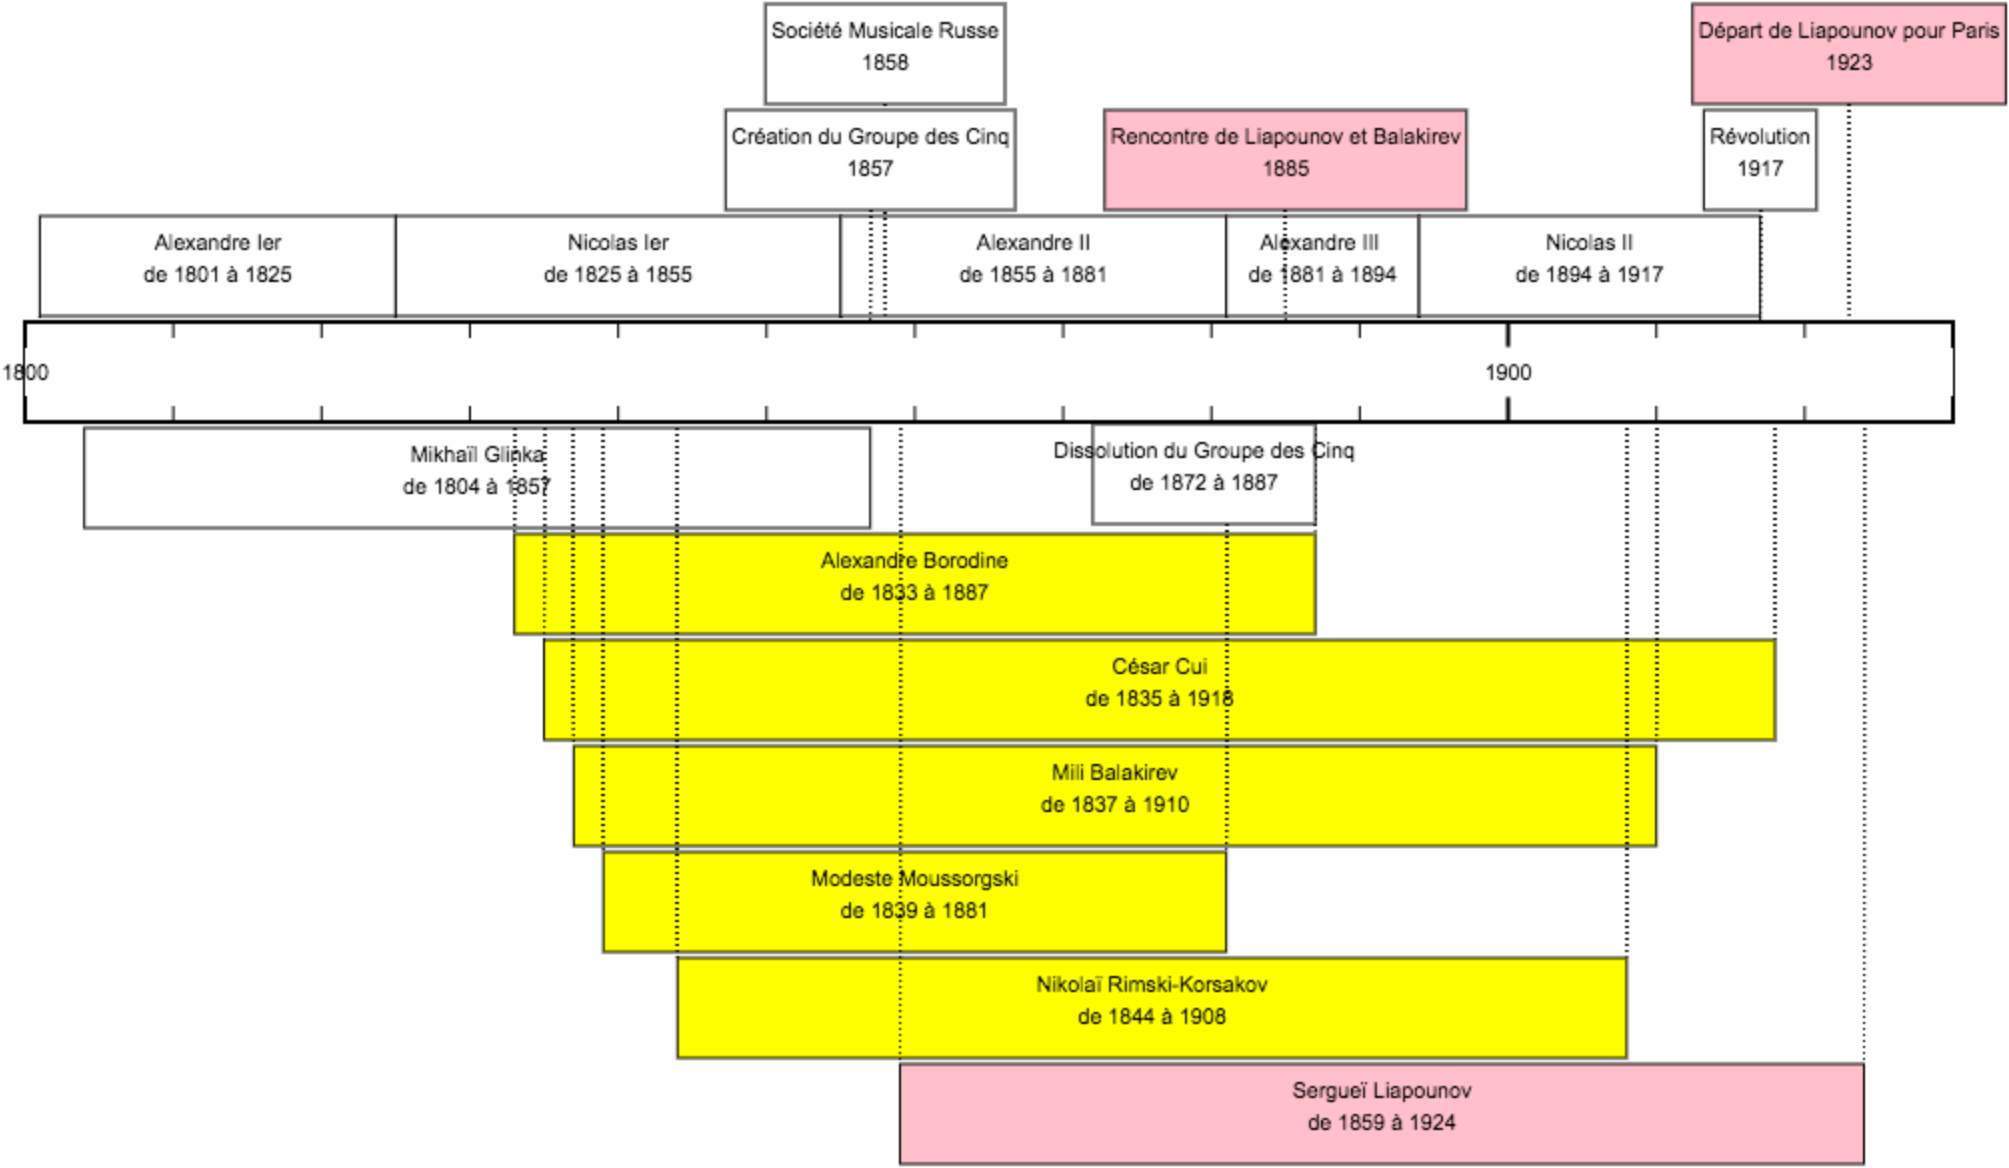
\includegraphics[width=15.5cm, keepaspectratio]{frise.png}
  \end{bigcenter}
  \caption{\label{frise}Frise chronologique des principaux événements depuis la naissance de Mikhaïl Glinka jusqu'à la mort de Sergueï Liapounov.}
\end{figure}

%%%%%%%%%%%%%%%%%%%%%%%%%%%%%%%%%%%%%%%%%%%%%%%%%%%%%%%%%%%%%%%%%%%%%%%%%%%%%

\chapter{L'œuvre de Sergueï Liapounov}

Ce chapitre est dédié à l'étude de la bibliographie et de l'œuvre Sergueï Liapounov. Plus particulière nous essayerons de positionner ce dernier face aux héritages du romantisme européen et face à l'idéal musical du groupe \emph{Groupe des Cinq}. Nous nous intéresserons plus particulièrement aux \emph{12 études d'exécution transcendante} qui sont typiquement russes de par leur couleurs slaves mais s'inscrivent dans la continuité des études éponymes de Franz Liszt. Finallement, nous essayerons de dégager les principales raisons de l'anonymat de ce compositeur qui semble pourtant laisser une marque importante dans l'histoire de la culture musicale russe\ref{onegina1}.

\section{La jeunesse du compositeur}

Sergueï Mikhaïlovitch Liapounov (ou Lyapunov) est un compositeur, pianiste virtuose, chef d'orchestre, éthnomusicologue, éditeur et pédagogue russe, né le 30 novembre 1859 à Iaroslavl\footnote{Iaroslavl est la capitale administrative de l'oblast de Iaroslavl. La ville est située au confluent de la Volga et de la Kotorosl, à 282 km au nord-est de Moscou.} et mort le 8 novembre 1924 à Paris. Son père, l'astronome Mikhail Vassilievitch Liapounov et sa mère Sofia Aleksandrovna Shilipova ont eu trois fils. L'aîné Alexandre Liapounov (1857-1918) est un célèbre mathématicien connu pour ses travaux sur l'étude des systèmes dynamiques (stabilité au sens de Liapounov). Le cadet Boris Lyapunov (1862–1943) est un linguiste spécialisé dans les langues slaves et membre de l'\emph{Académie des Sciences}.

Le talent musical de Liapounov se manifeste très tôt. Encore incapable de parler, il réclame le piano. Âgé de quatre ans et accompagné de son fère Alexandre, il reçoit ses premiers cour de piano de sa mère, une femme instruite un bonne pianiste. Après la mort prématurée du père en 1868, la famille Liapounov s'installe à Nijni Novgorod\footnote{Nijni Novgorod est capitale administrative de l'oblast de Nijni Novgorod et centre économique de la région économique de Volga-Viatka. La ville est située au confluent de la Volga et de l'Oka, à 405 km à l'est de Moscou.}. Liapounov prend des cours de piano par l'intermédiaire de l'antenne de Nijni Novgorod de la \emph{Société Musicale Russe}. A cette époque, il s'implique dans des conserts étudiant et interprète publiquement des œuvre de Bach, Haydn, Beethoven et Mendelssohn. A la fin de ses études et sur les recommandations de Nikolaï Rubinstein lui même, il s'inscrit en 1878 au conservatoire de Moscou. Ses principaux professeurs sont Karl Klindworth et Paul Pabst (deux anciens élèves de Franz Liszt) pour le piano et Sergueï Taneïev et Piotr Tchaïkovski pour la composition.

En 1883, lorsque Liapounov termine ses études, il est devenu un véritable virtuose\footnote{Sa fille, Anastasia Liapounov, a laissé une des rares descriptions sur le jeu pianistique de son père : « ... la simplicité du phrasé avec une variété considérable de sonorités. Son jeu était simple, noble, calme, peut-être même trop équilibré .... ».}. Son catalogue d'œuvres jouées est important et compte des pièces de difficultés considérables. A titre d'exemple, on peut citer les concertos de Chopin ou encore le diabolique \emph{Islamey} de Balakirev. Cependant, il ne se destine pas à une carrière de concertiste. De ses aveux même, il ne se concidère pas comme un pianiste majeur, le jeune pianiste manque de confiance en lui sur scène. Il refuse le post d'enseignant offert par Nikolaï Rubinstei estimant que « la vraie route qui doit passer par la musique russe ». En effet, il développe un sentiment de rejet à l'égare de l'école de Moscou et de Tchaïkovski. C'est à ce moment qu'il rencontre Mili Balakirev pour la première fois. Le jeune compositeur prend la décision ferme d'adhérer au \emph{Groupe des Cinq}. En 1885, il s'établi à Saint Pétersbourg.

C'est durant les années 1880 que Liapounov compose ses prémières œuvres sérieuses. L'influence de la musique de Chopin et Liszt est très marquée. A titre d'exemple, citons la valse op. 1 (voir figure \ref{op1}) ou encore \emph{Rêverie du soir}, op. 3 (voir figure \ref{op3}) où il est intéressant de noter la couleur orientable des premières mesures. Le nocturne op. 8, écrit quelques années plus tard, est un très bel hommage à la musique de Chopin.

\begin{figure}[!ht]
  \begin{bigcenter}
    \begin{tabular}{lr}
      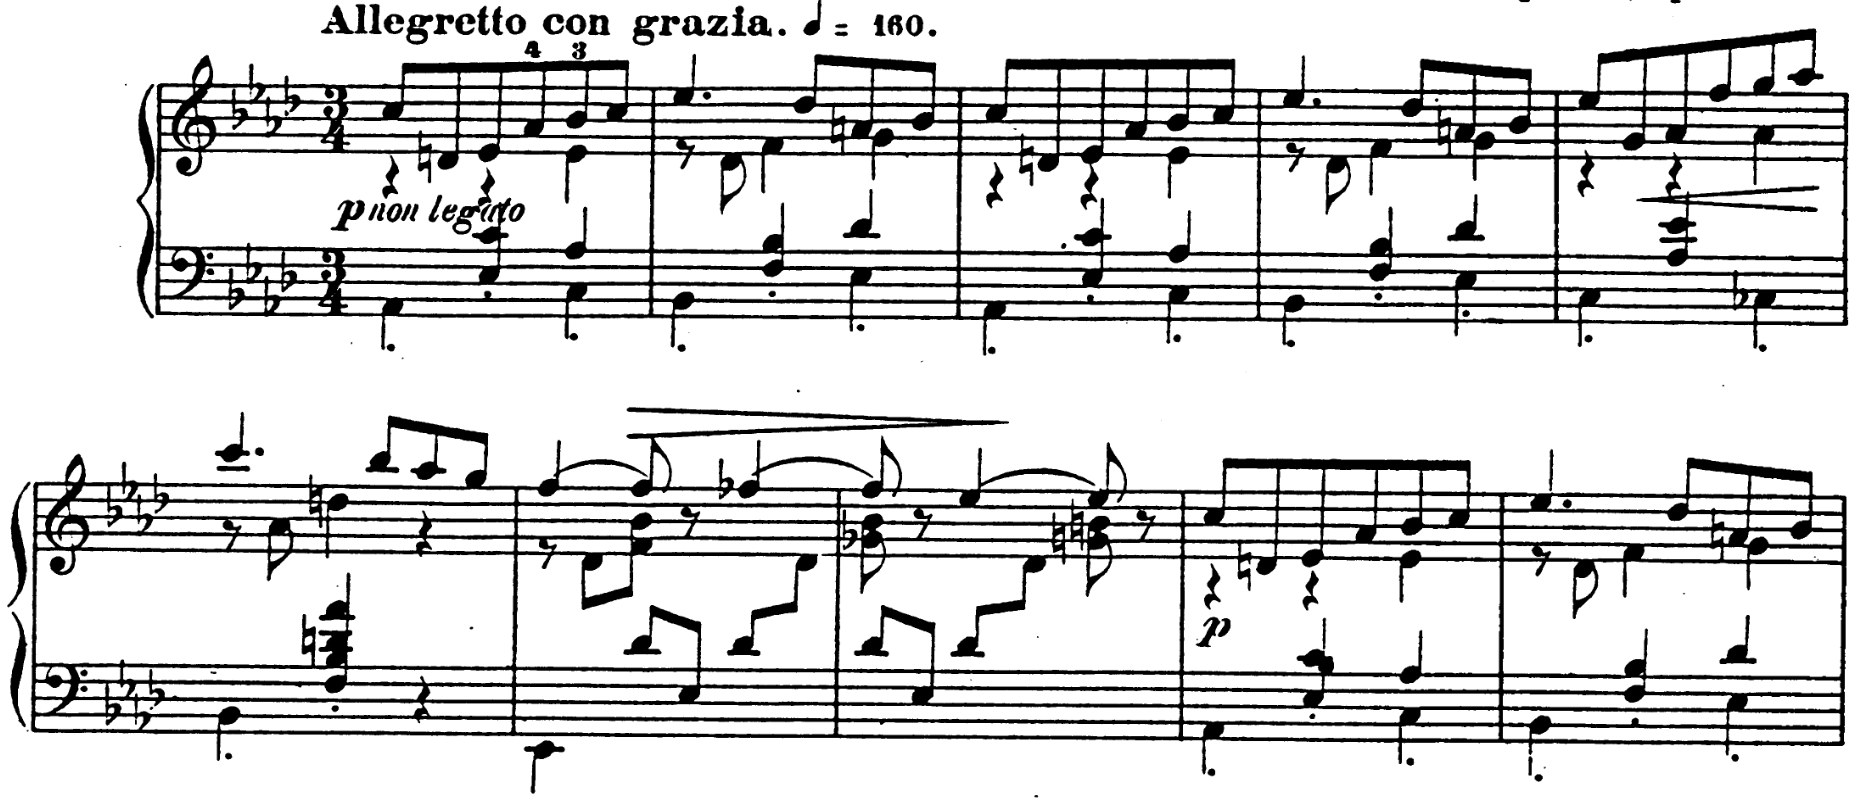
\includegraphics[width=12.5cm, keepaspectratio]{op1.png}
      &
      
\includegraphics[width=3cm, keepaspectratio]{op1-qr.png}
    \end{tabular}
  \end{bigcenter}
  \caption{\label{op1}Extrait de \emph{Trois Morceaux} op. 1 \no 3 (valse).}
\end{figure}

\begin{figure}[!p]
  \begin{bigcenter}
    \begin{tabular}{lr}
      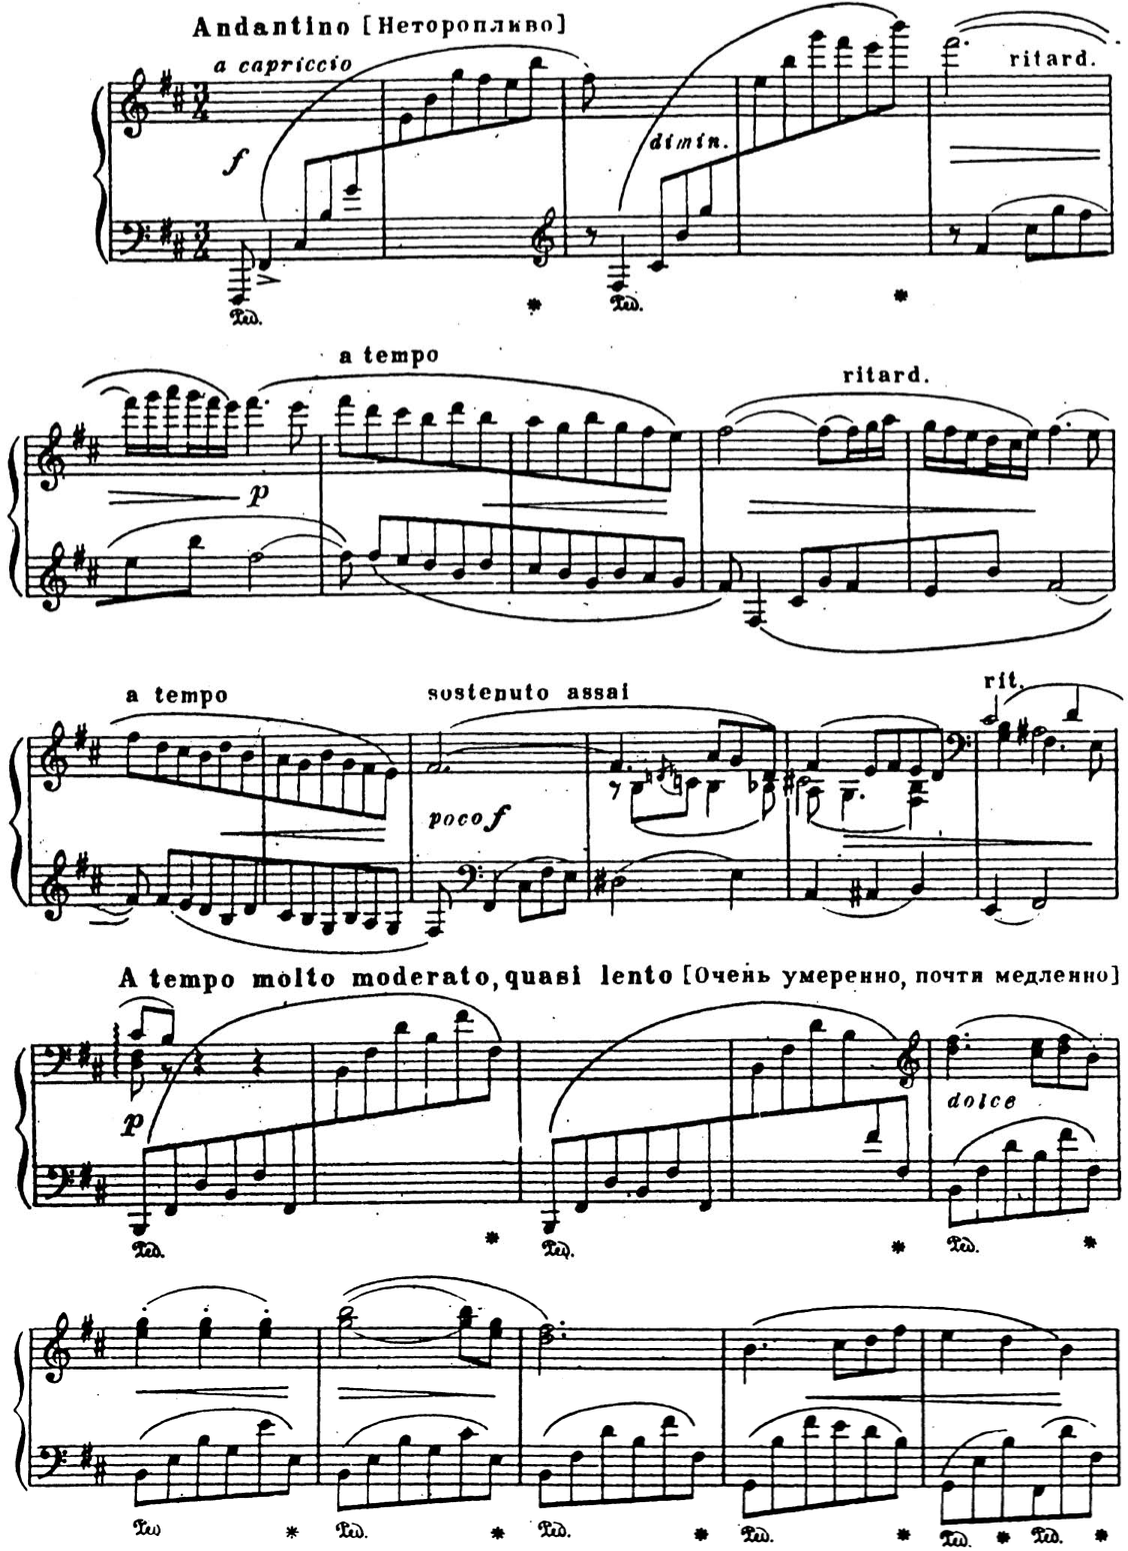
\includegraphics[width=12.5cm, keepaspectratio]{op3.png}
      &
      
\includegraphics[width=3cm, keepaspectratio]{op3-qr.png}
    \end{tabular}
  \end{bigcenter}
  \caption{\label{op3}Extrait de \emph{Rêverie du soir} op. 3.}
\end{figure}

\begin{figure}[!p]
  \begin{bigcenter}
    \begin{tabular}{lr}
      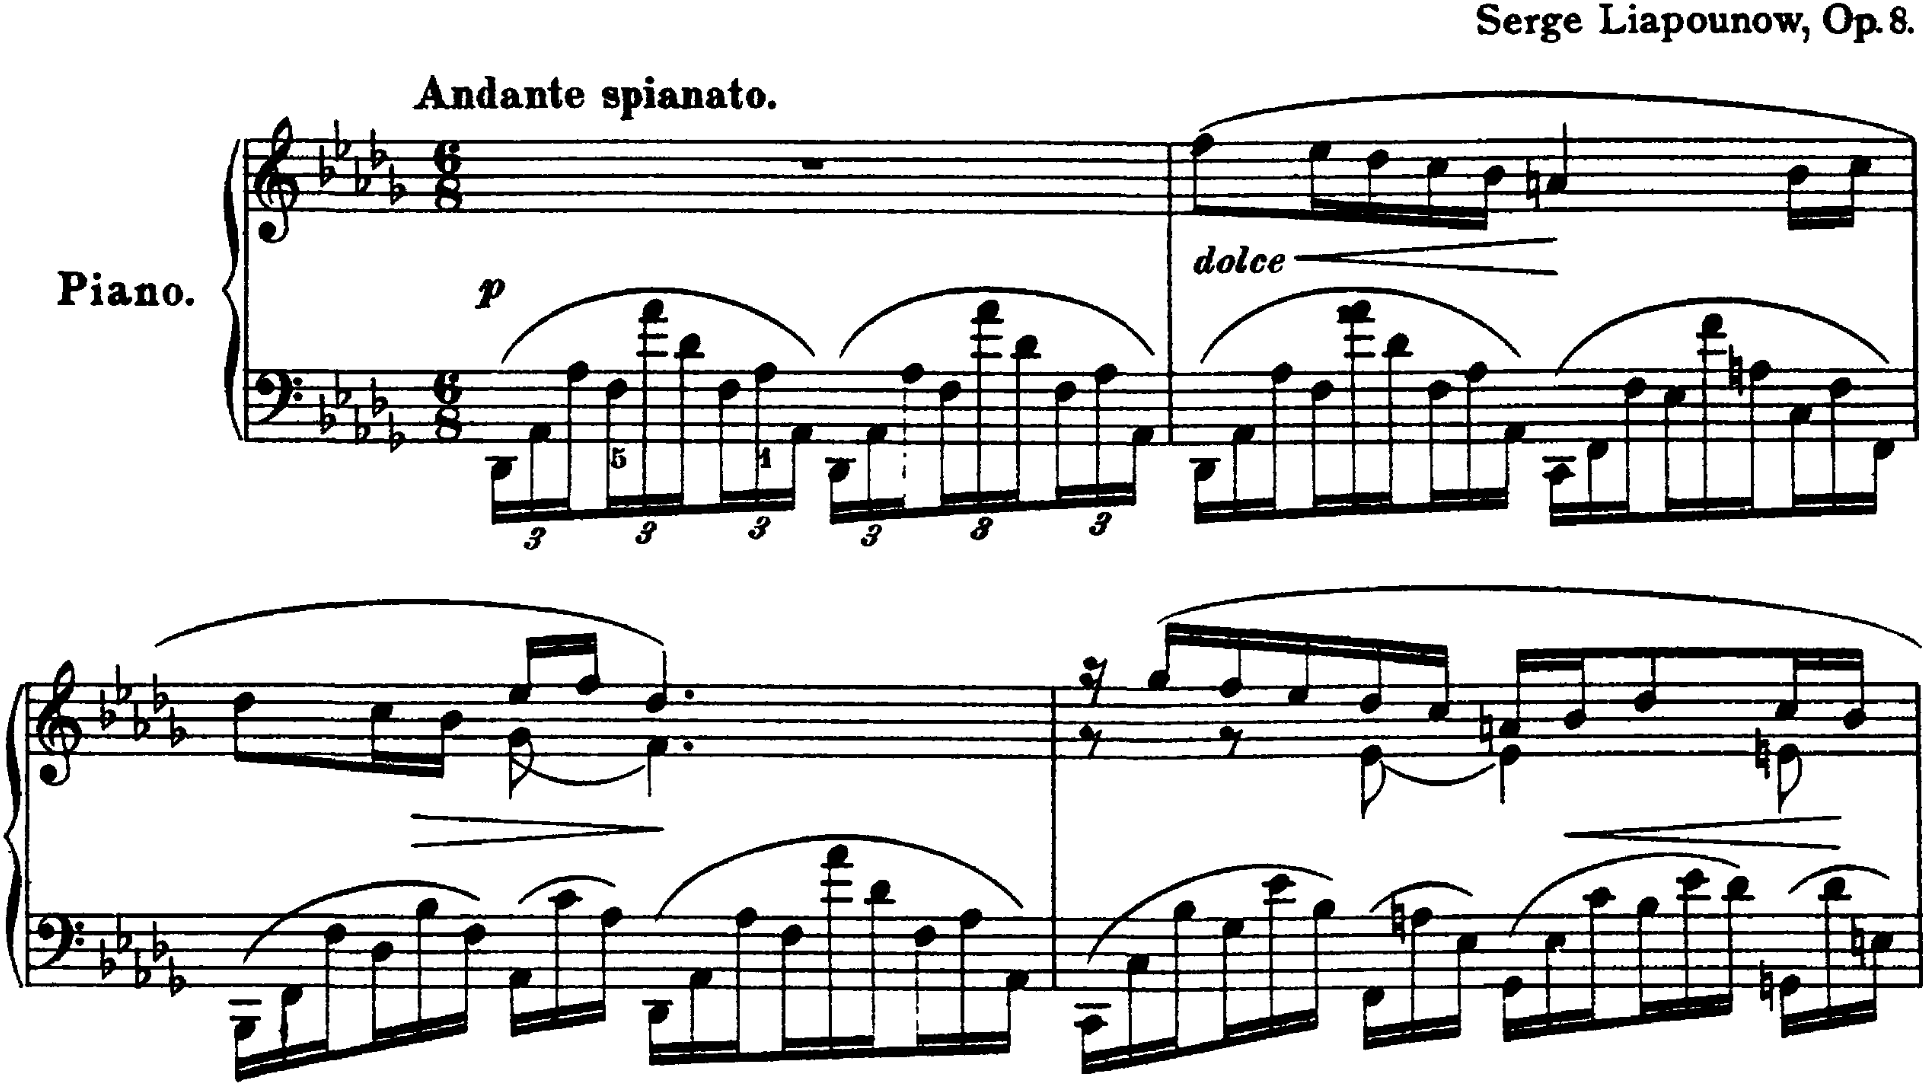
\includegraphics[width=12.5cm, keepaspectratio]{op8.png}
      &
      
\includegraphics[width=3cm, keepaspectratio]{op8-qr.png}
    \end{tabular}
  \end{bigcenter}
  \caption{\label{op3}Extrait du \emph{Nocture} op. 8.}
\end{figure}

\section{Liapounov et Balakirev}

TODO

\newpage
\newpage

\section{Les \emph{études d'exécution transcendante} op. 11}

Composées entre 1897 et 1905, les 12 \emph{études d'exécution transcendante} op. 11 de Liapounov représentent sans aucun doute le sommet de son art. Cette œuvre reste malheureusement fort peu connu tant des interprètes que des musicophiles. Ce monumental cycle d'études, environ 130 pages, est un vibrant hommage à la troisième révision (1852) des 12 \emph{études d'exécution transcendante} de Franz Liszt. La dernière étude \emph{Élégie à Franz Liszt} confirme définitivement l'hommage. Concernant les tonnalités, là où Liszt progresse par ton - ton relatif sur les touches blanches (do M - la m, fa M - ré m, etc...), Liapounov progresse sur les touches noires à partir de fa$\sharp$ M (fa$\sharp$ M, ré$\sharp$ m, etc...). Ainsi, les études de Liapounov se présentent clairement comme un complément des études de Liszt, les 24 tonnalités sont traitées.

\subsection{Similarités thématiques et textuelles}

Les études de Liapounov présentents des similarités plus ou moins évidentes avec leurs grandes sœurs. Le cas le plus évident concerne l'étude \emph{La ronde des sylphes} (\no 11) dont le nom évoque déjà \emph{La ronde des Lutins} chez Liszt. Le parallèle avec \emph{Feux follets} (\no 5) est immédiat : même tempo, même mesure, même dynamique (Allegretto chez Liszt, Allegretto scherzando chez Liapounov). Les éléments thèmatiques n'étant qu'une variation de ceux de l'étude originale (voir figure \ref{op11-xi}).

De façon similaire, il est textuellement évident d'associer \emph{Carillon} (\no 3) et \emph{Harmonie du soir} : écriture en choral, registre médium, cloches, \emph{Harpes éoliennes} (\no 9) et \emph{Chasse neige} (\no 12) : mesure ternaire et trémolos. Il est de plus légitime de raprocher \emph{Nuit d'été} (\no 5) et \emph{Ricordanza} (\no 9), \emph{Tempête} (\no 6) et \emph{l'étude en fa m} (\no 10), \emph{Idylle} (\no 7) et \emph{Paysage} (\no 3) puis enfin \emph{Chant épique} (\no 8) et \emph{Eroica} (\no 7).

\begin{figure}[!p]
  \begin{bigcenter}
    \begin{tabular}{lr}
      \vspace*{0.0cm}
      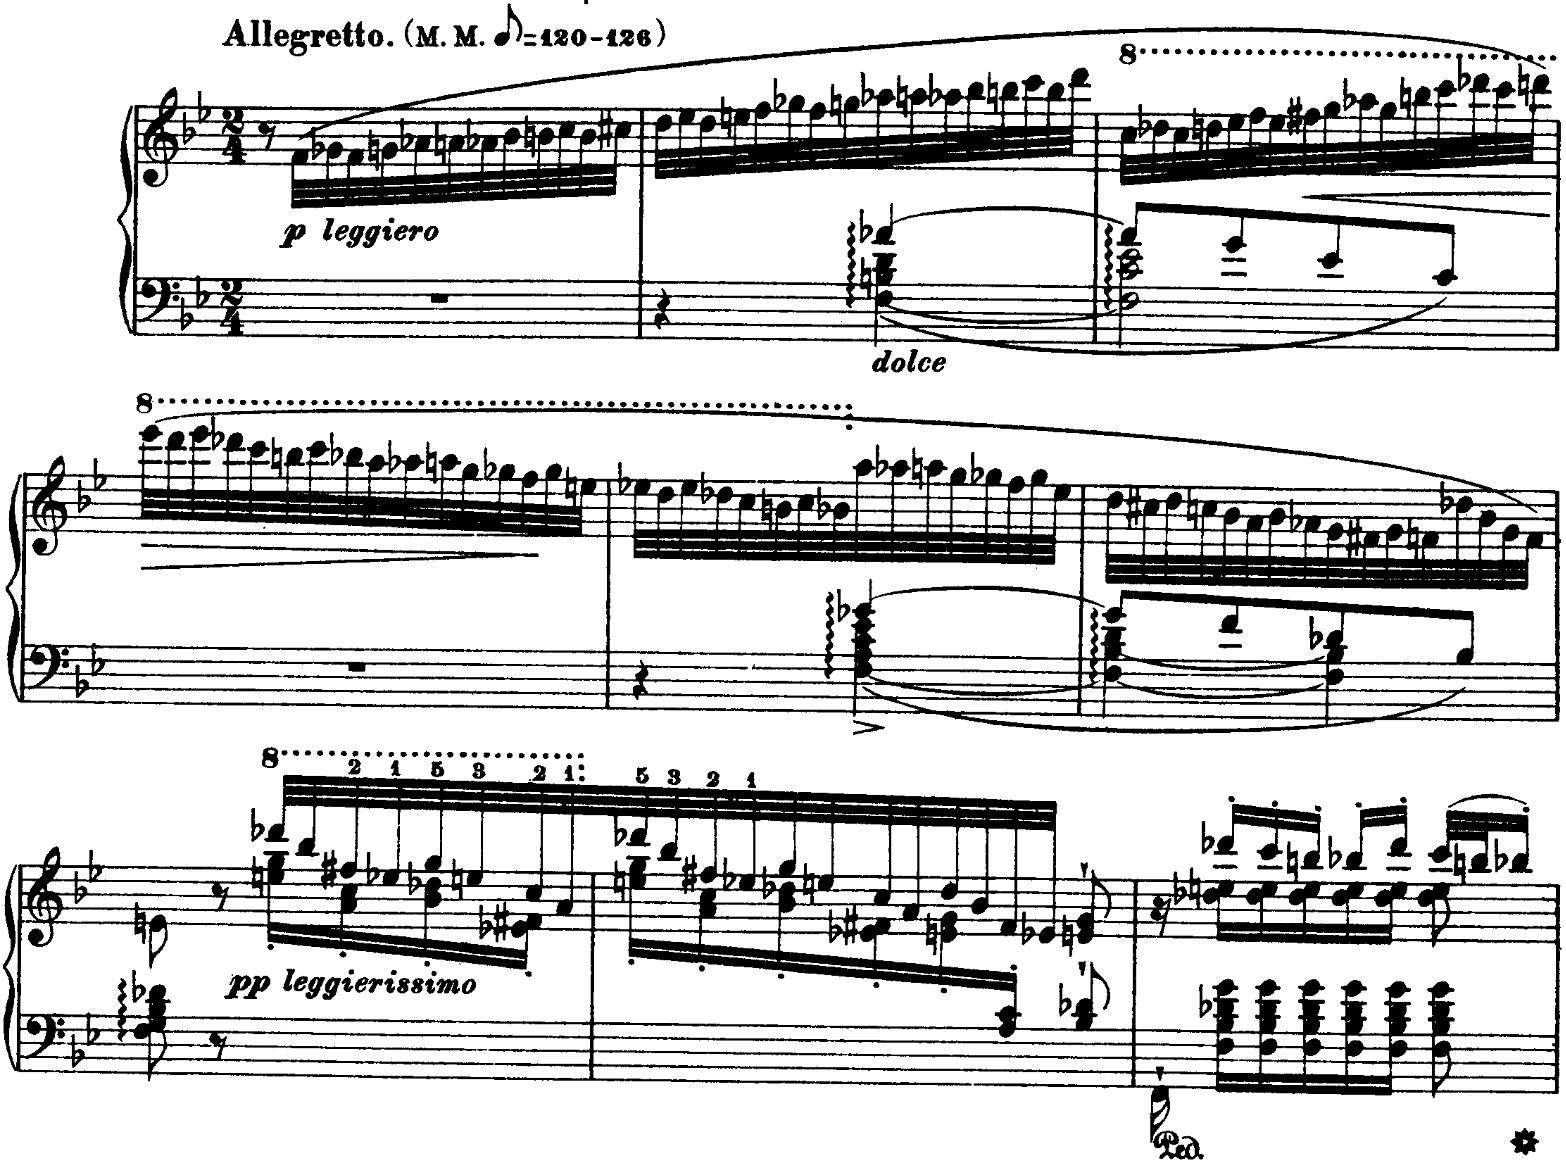
\includegraphics[width=12.5cm, keepaspectratio]{feux-follets.png}
      &
      
\includegraphics[width=3cm, keepaspectratio]{feux-follets-qr.png}
      \\
      \vspace{0.5cm} &
      \\
      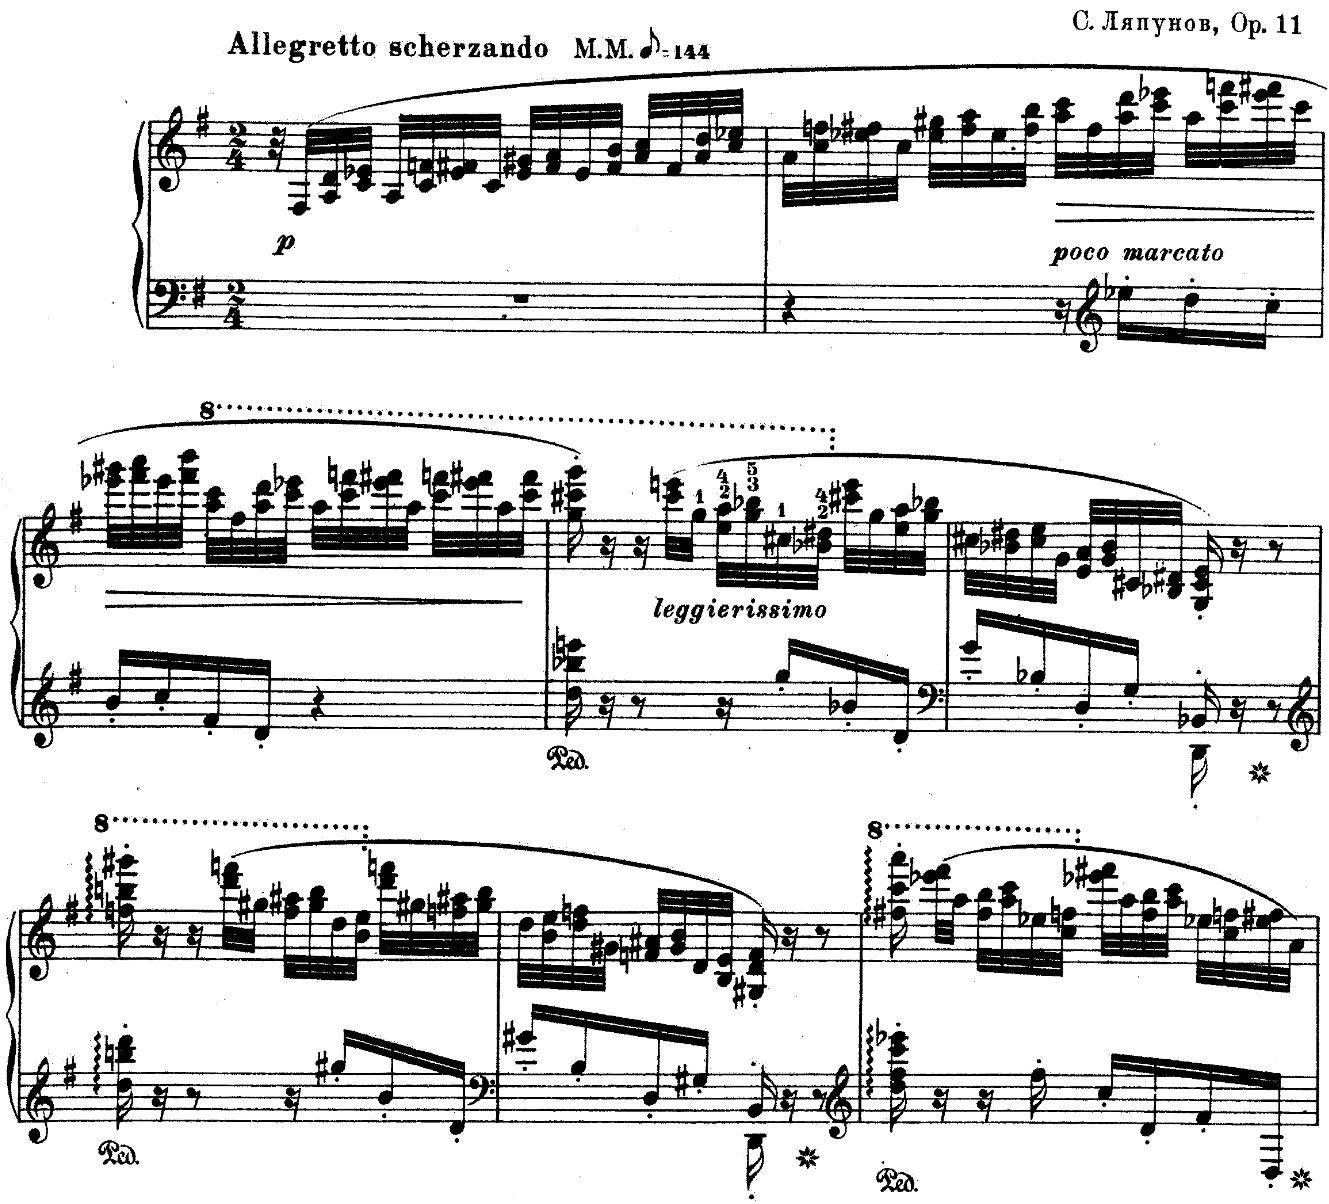
\includegraphics[width=12.5cm, keepaspectratio]{op11-xi.png}
      &
      
\includegraphics[width=3cm, keepaspectratio]{op11-xi-qr.png}
    \end{tabular}
  \end{bigcenter}
  \caption{\label{op11-xi}Comparaison des début de \emph{Feux follets} de Liszt (en haut) et de \emph{La ronde des sylphes} de Liapounov (en bas).}
\end{figure}

\subsection{Une \emph{musique à programme}}

Il existe un autre point commun entre Liapounov et Liszt, leur intéret pour la \emph{musique à programme} (expression inventé par Liszt lui-même). Pour une œuvre purement instrumentale, le \emph{programme} consiste en l'ajout qu'un texte d'intention par lequel le compositeur explicite ses thèmes d'inspiration afin de « préserver son œuvre de l'arbitraire d'une explication poétique erronée et d'orienter par avance l'attention sur l'idée poétique du tout ou sur un point particulier ».

Les études de Liapounov sont un bel exemple de \emph{musique à programme}. Chacune d'entre elles disposent d'un titre évocateur en français, deux d'entre elles sont accompagnés d'un poëme (Carillon et Térek) et une autre (Chant épique) est inpirée du chant populaire \emph{Iz-za lesu, lesu temnogo} (Sorti des bois, sombres bois). 

\subsection{Sources d'inspiration russes}

Si de nombreux éléments rapprochent les études des deux compositeurs, il en est un qui singularise les études de Liapounov : l'empoi de matériaux typiquement russes. Comme nous le verrons plus loin, les références (et citations) à Balakirev, Borodine, Morssorski et Rimsky-Korsakov sont très présentes. L'amour du compositeur pour les traditions folkloriques anciennes, pour l'Eglise orthodoxe (\emph{Carillon}) et pour la littérature russe affect profondément le caractère des études de Liapounov (\emph{Carillon}, \emph{Térek}, \emph{Chant épique}, \emph{Lesghinka}) et les singularise par rapport à celles de Liszt.

\subsection{Brève analyse de l'œuvre}

\begin{tabular}{ll}
  \raisebox{-0.5cm}{
\includegraphics[width=3cm, keepaspectratio]{op11-qr.png}}
  &
  
\includegraphics[width=2cm, keepaspectratio]{hp.png}
\end{tabular}

Dans cette sous-section, nous donnons une très brève analyse de l'œuvre.

\subsubsection{I \emph{Berceuse} (1897-1898)}

La première étude est un Andantino à 4/2 de forme intro + A=(ab) + A'=(a'b') varié qui évoque, de par sa pédale de fa$\sharp$ majeur et sa mélodie, la \emph{Berceuse} op. 57 en ré$\flat$ M de Chopin. Le style global est similaire à celui des nocturnes de Field ou Chopin mais le thème est d'inspiration russe.

\subsubsection{II \emph{La ronde phantômes} (1897-1898)}

La deuxième étude est un Presto à 6/8 en ré$\sharp$ m, très virtuose et accidenté, de forme intro + A=(ab) + A'=(a'b') + coda. Avec ses triplets de huit croches, il alterne une écriture en accords brisés en miroir aux deux mains pour (a) avec un motif plus lyrique pour (b). Le caractère modal de (a), issu du folklore et de la musique liturgique donne un caractère distinctement russe à cette étude.

\subsubsection{III \emph{Carillon} (1901)}

La troisième étude est accompagnée de son programme descriptif :\\

« On entend l'appel d'une cloche et les sons d'un chant d'église. Le son des cloches augmente et grandi graduellement; les petites cloches se réunissent à la grande et se confondent dans un carillon général. Alternativament, se font entendre les chants solennels de l'église et les sons des cloches s'unnissant enfin dans un choeur imposant que couvrent les coups lours de la grande cloche. »

Elle fut vraisemblablement composée à partir des matériaux recueillis par Liapounov lors de l'expédition de 1893. Son caractère descriptif Allegro moderato e maestoso ainsi que son caractère orchestral la rapproche de \emph{La Grande Porte de Kiev} des \emph{Tableaux d'une exposition} de Moussorgski.

\subsubsection{IV \emph{Térek} (1900)}

La quatrième étude est accompagnée d'un poëme de Mikhaïl Lermontov\footnote{Il s'agit ici d'une traduction du russe vers l'anglais réalisée par Igor Chernyshev. L'édition Zimmermann, utilisée pour ce mémoire, ne contient qu'une traduction du russe vers l'allemand.} :\\

\begin{tabular}{ll}
\hspace{-3.9mm}« Térek moans, wild and wicked,
&
Scattering through the plains,
\\
Among steep mountains,
&
He appears cunning,
\\
Like a cry of a storm,
&
And in sweet adulation,
\\
Whose tears are airborne.
&
Murmurs at the Caspian Sea. »
\end{tabular}\\

Cette étude est un double portait. Le Terek\footnote{D'une longueur de 623 kilomètres, il coule sur les territoires de la Géorgie et de la Russie et se jette dans la mer Caspienne.}, un des principaux fleuves du Caucase, est dépeint de façon violente, agitée et sauvage (voir figure \ref{op11-iv} en haut) alors que l'utilisation d'un des thème des \emph{Danses polovtsiennes} de l'opéra \emph{Le Prince Igor} de Borodine évoque la tranquilité de la mer Caspienne. Notons que l'intrique du célèbre poèmes symphoniques \emph{Tamara} de Balakirev, inspiré d'un poème de Lermontov, se déroule sur les bords du fleuve Térek. Cette étude est un hommage de Liapounov à son maître.

\begin{figure}[!p]
  \begin{bigcenter}
    \begin{tabular}{lr}
      \vspace*{0.0cm}
      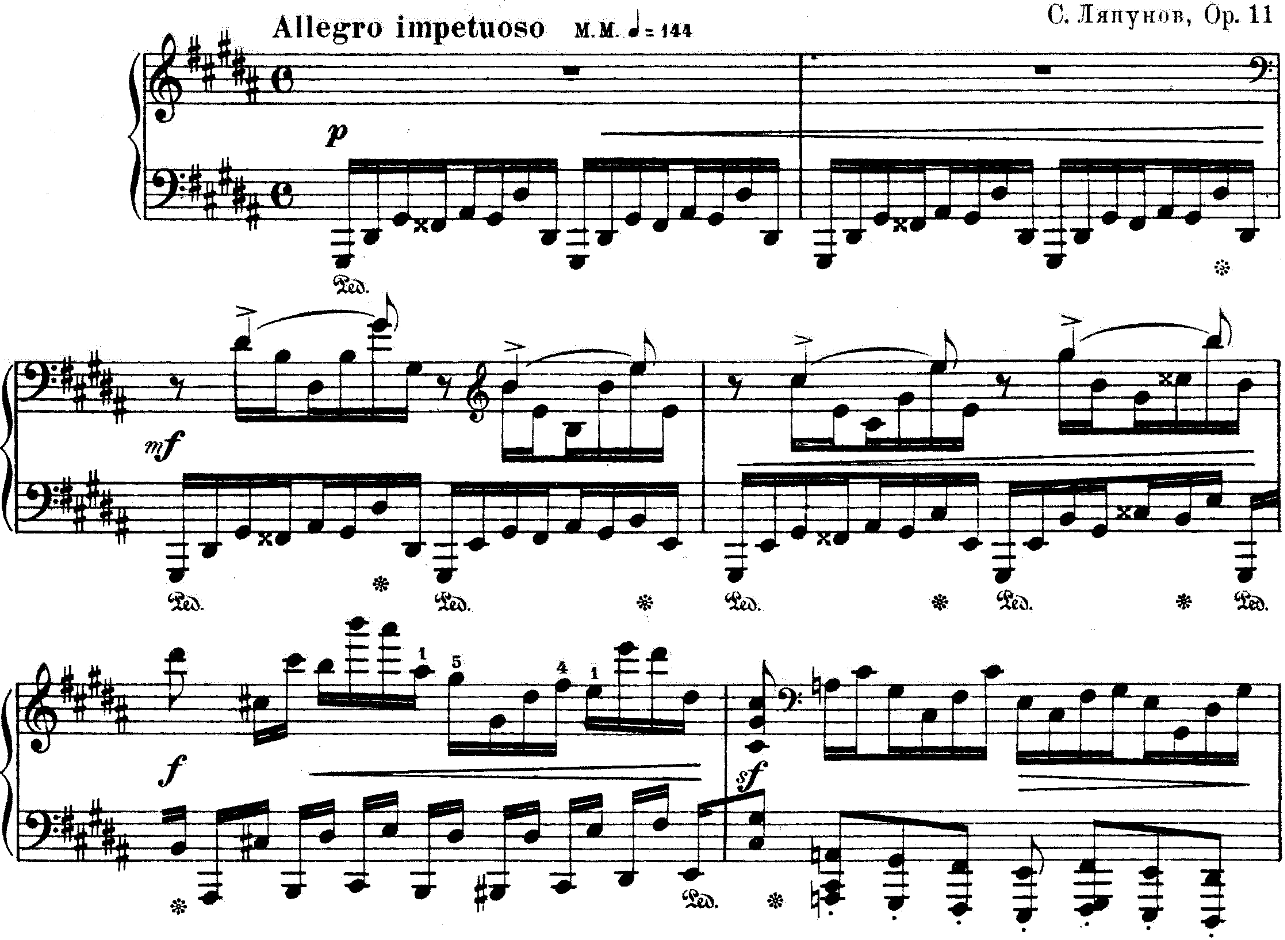
\includegraphics[width=12.5cm, keepaspectratio]{op-11-iv-1.png}
      &
      
\includegraphics[width=3cm, keepaspectratio]{op-11-iv-qr.png}
      \\
      \vspace{0.5cm} &
      \\
      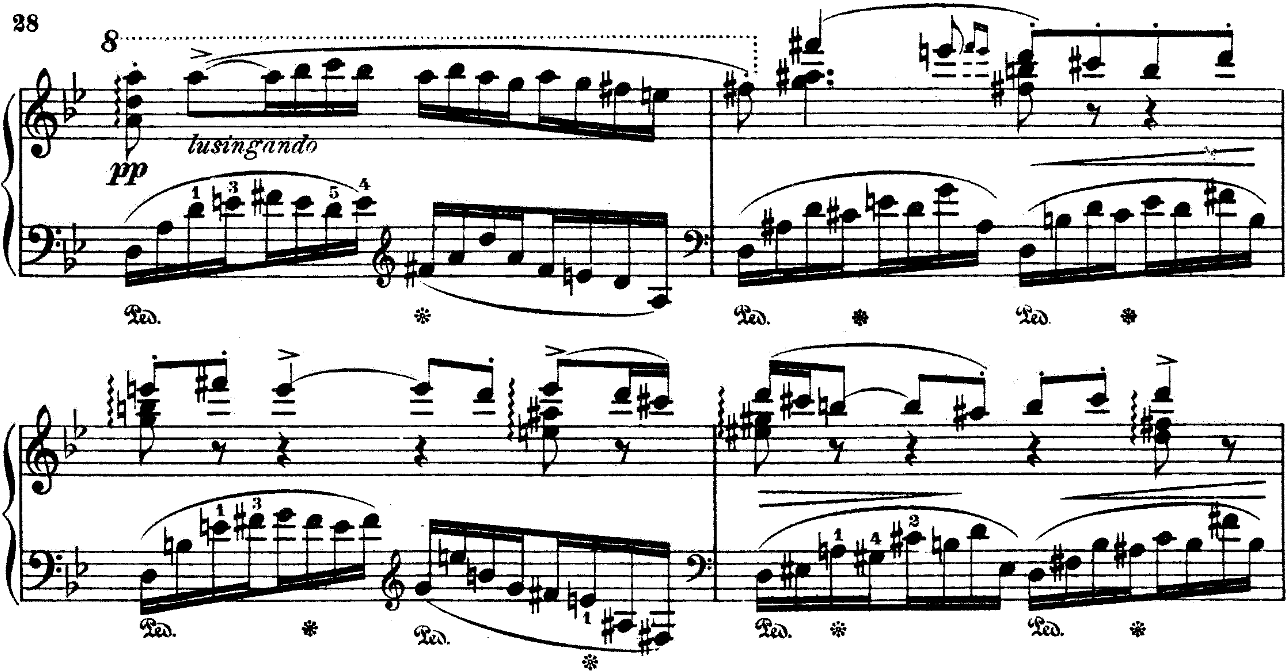
\includegraphics[width=12.5cm, keepaspectratio]{op-11-iv-2.png}
      &
      
\includegraphics[width=3cm, keepaspectratio]{op-11-iv-qr.png}
    \end{tabular}
  \end{bigcenter}
  \caption{\label{op11-iv}Début de \emph{Térek}, l'agitation est asociée à la violence et aux cotés sauvages du fleuve (en haut) et citation des \emph{Danses polovtsiennes} de l'opéra \emph{Le Prince Igor} de Borodine, entre autre, mesure 28, pour évoquer la tranquilité de la mer Caspienne (en bas).}
\end{figure}

\subsubsection{V \emph{Nuit dété} (1900)}

La cinquième étude est le pendant liapounesque de l'étude \emph{Ricordanza} de Liszt. Lento ma non troppo, écrite à 6/8 au lieu de 6/4 et avec quatre dièses (mi M) au lieu de quatre bémoles (la$\flat$ M), il s'agit d'une grande forme libre de près de huit minutes.

\subsubsection{VI \emph{Tempête} (1897)}

La sixième étude est un Allegro agitato molto à 2/4, en do$\sharp$ m, également très virtuose et accidenté. Elle a globalement pour forme A=(abc) + A'=(a'b'c') + coda. Pour le caractère, la section (a) renvoie à l'étude \no 11 op. 25 de Chopin (\emph{Vent d'hiver}) ainsi qu'à \emph{Orage} dans le premier cahier des \emph{Années de pèlerinage} de Liszt. D'un point de vu thématique, a et b semblent respectivement mélodiquement et graphiquement s'inspirer de l'\emph{étude en fa m} des \emph{études d'exécution transcendante} de Liszt.

\subsubsection{VII \emph{Idylle} (1901)}

La septième étude est un Andantino pastorale à 6/8, en la M, de forme A=(aa') + B + A'=($\sim$ a). D'un caractère relativement contrapointique, elle peut évoquer \emph{Paysage} des \emph{études d'exécution transcendante} de Liszt (fa M). Peut-être cette pièce fut inspirée par le village de Bolobonovo près de Iaroslavl où Liapounov a passé son enfance.

\subsubsection{VIII \emph{Chant épique} (1903)}

La huitième étude s'impire du chant populaire \emph{Iz-za lesu, lesu temnogo} (Sorti des bois, sombres bois), collécté lors de l'expédition de 1893 et publié dans l'ouvrage \emph{Songs of the Russian People} (voir figure \ref{woods}) :\\

\begin{tabular}{ll}
\hspace{-3.9mm}« Out of the woods
&
Behind the crest
\\
  \quad{}Dark woods.
&
  \quad{}The White Tzar leads,
\\
Out of the mountain,
&
And after Himself he leads
\\
  \quad{}Steep mountain.
&
  \quad{}His mighty legions,
\\
It was not the white dawn
&
His forces,
\\
  \quad{}That appeared,
&
  \quad{}And not small ones.
\\
It was not the red sun
&
Not small forces
\\
  \quad{}That rose.
&
  \quad{}But forty-three regiments.
\\
There appeared rather
&
Forty-three regiments,
\\
  \quad{}The Tzar’s crest.
&
  \quad{}Dense with soldiers.
\\
The crest of the Tzar
&
All the soldiers
\\
  \quad{}Of the Emperor.
&
  \quad{}Who are new recruits. »
\end{tabular}\\

Il s'agit d'une \emph{byline}, une chanson narrative héroïque de la Russie ancienne. Elle dépeint une lutte épique du peuple russe contre les envahisseurs - des Mongols du Sud aux Vikings du Nord -. Dans son étude, Liapounov concerve la tonalité de fa$\sharp$ m et la mesure C devient C\hspace{-2mm}| pour plus de dynamique. La tête du chant apparait dés la première mesure.\\

Remarque : On peut noter une certaine similarité entre le thème \emph{Iz-za lesu, lesu temnogo} et le chant populaire russe utilisé dans les \emph{Variations et Fugue sur un thème russe} op. 49.

\begin{figure}[!ht]
  \begin{bigcenter}
    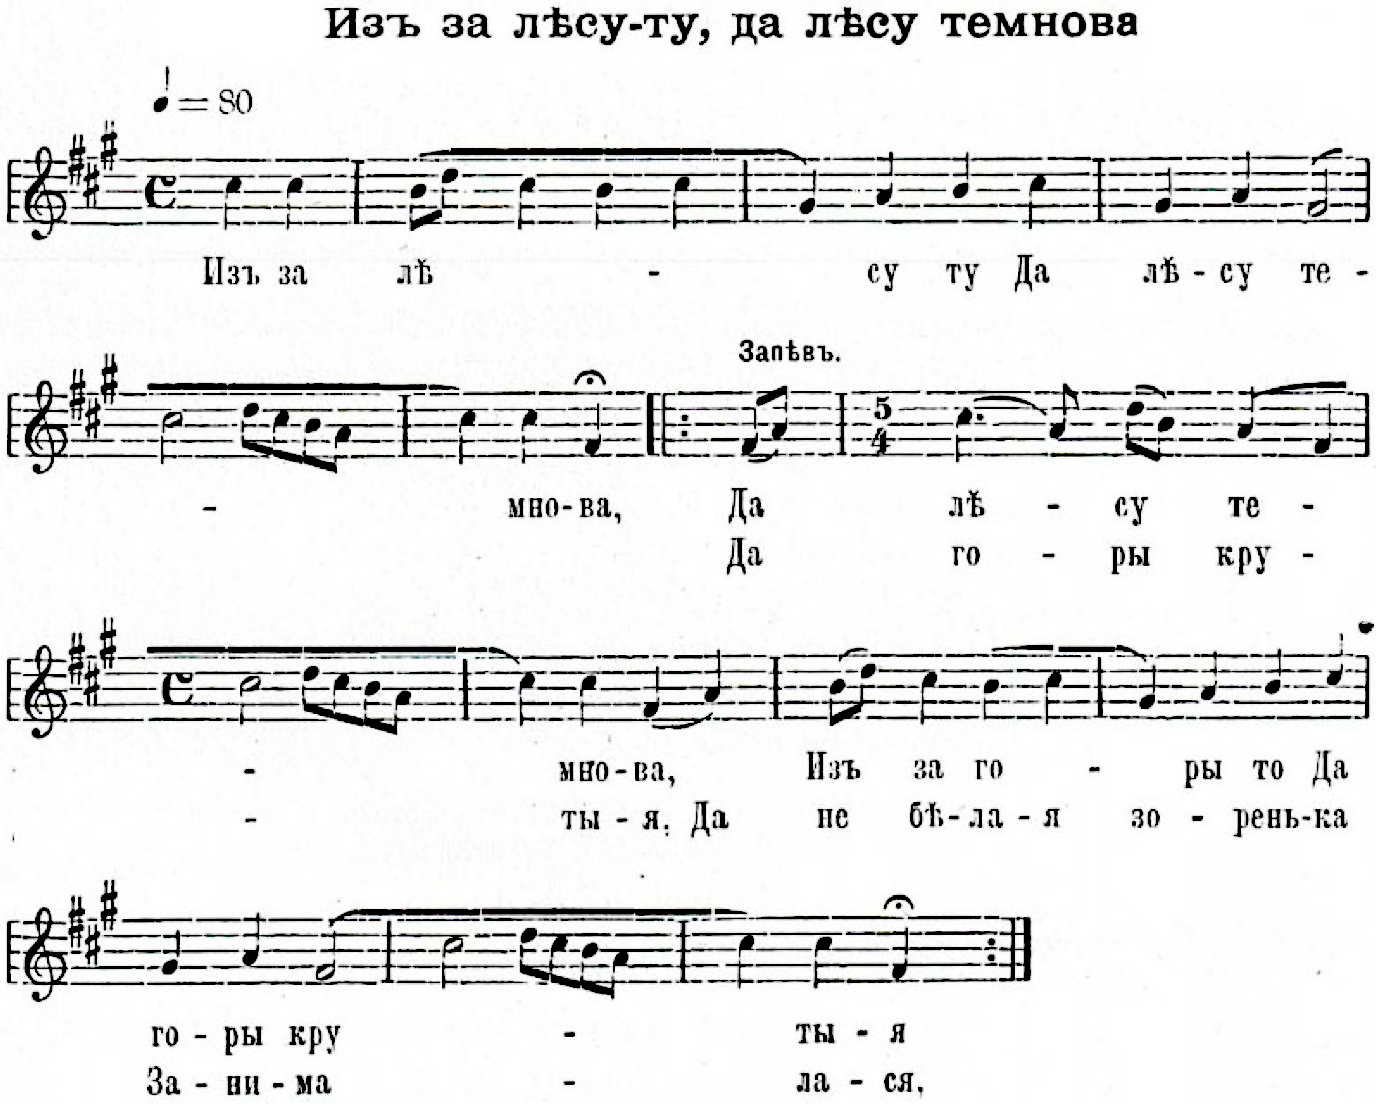
\includegraphics[width=12.5cm, keepaspectratio]{woods.png}
  \end{bigcenter}
  \caption{\label{woods}Chant populaire \emph{Iz-za lesu, lesu temnogo} (Sorti des bois, sombres bois) collécté lors de l'expédition de 1893 et publié dans l'ouvrage \emph{Songs of the Russian People}.}
\end{figure}

\subsubsection{IX \emph{Harpes éoliennes} (1902)}

La neuvième étude est un Adagio non tanto à 9/8, en si m, de forme A + cadence + B + cadence + C. Elle porte le même nom que la première étude op. 25 de Chopin. La pièce est constuite sur l'usage d'un élément thématique utilisé de façon récurrente. L'usage extrêmement vituose des trémolots est un hommage à \emph{Chasse neige} des \emph{études d'exécution transcendante} de Liszt (si$\flat$ m).

\subsubsection{X \emph{Lesghinka} (1903)}

La partition complète de cette étude est fournie dans en l'annexe 1.

\subsubsection{XI \emph{La ronde des sylphes} (1905)}

La onzième étude est un Allegretto scherzando non tanto à 2/4, en sol M, de forme tripartite. Comme indiqué précédemment, elle reprend les thèmes, le caractère et les difficultés téchniques de l'étude \emph{Feux follets} en si$\flat$ M de Liszt (voir figure \ref{op11-xi}).

\subsubsection{XII \emph{Elégie en Mémoire de François Liszt} (1905)}

La douzième étude, en mi m, est à la fois la dernière et la plus monumentale des études du recueil. Sa durée d'exécution approche les 12 minutes. Elle est écrite sur le modèle des \emph{Rhapsodies hongroises} de Liszt auxquelles elle empreinte au passage de nombreux éléments thématiques (en particulier à la première). La forme est libre, en un seul mouvement et, comme chez Liszt, assez proche de la fantaisie.

\subsubsection{Conclusion}

Au moment de sa publication en 1905, l'opus 11 de Liapounov est le plus grand cycle d'études pour piano après les opus 10 et 25 de Chopin et les \emph{études d'exécution transcendante} de Liszt. Il s'agit d'un très bel hommage à ce dernier, le dédicataire de l'œuvre. L'hommage au groupe des cinq, et plus particulièrement à Balakirev et Borodine (\emph{Térek} et \emph{Lesghinka}, etc...), est également très fortement marqué.

Ces études présentent un fort intéret pédagogique mais ne se limitent pas à la virtuosité. Au contraire, elles redémontrent les capacités du piano à rendre de riches couleurs orchestrales. Certaines études sont de vraies peintures sonores.

Comme le faisait Liszt, certaines des études de Liapounov sont accompagnées d'éléments programmatiques. Ces derniers servent à caractériser le premier thème tandis de le(s) suivant(s) rendent compte, avec contraste, des impressions plus personnelles du compositeur.

Les très nombreuses références au folklore russe ainsi que la référence au romantisme européen positionnent ces études dans la continuité de travaux et des idéaux du groupe des cinq. Même s'il demeure peu connu de nos jour, l'opus 11 de Liapounov constitue le somment de la musique de Liapounov et un chef-d'œuvre de la musique russe. 

%%%%%%%%%%%%%%%%%%%%%%%%%%%%%%%%%%%%%%%%%%%%%%%%%%%%%%%%%%%%%%%%%%%%%%%%%%%%%
